

\newchapter{Исчисление остатков}


\section{Арифметика остатков}

\subsection{Конспект}
\begin{enumerate}\setlength{\itemsep}{1pt}
\item Рассмотрим бытовую задачу. Вам нужно выключить печку через 40 минут, но у вас нет таймера, зато есть будильник, на котором можно выставить время звонка. Сейчас 12:30, на какое время требуется поставить будильник? Ответ: 13:10. Почему так? Дело в том, что в часе 60 минут, и если к 30 минутам прибавить 40, получается 70 минут, что больше часа. Поэотму добавляем 1 час и остаток --- 10 минут.
\item Еще пример: сколько часов будет через 20 часов, если сейчас 8 утра? Можно решать аналогично: $8+20=28$, затем убираем полные сутки, т.е. 24 часа, остается 4 часа утра.
\item Можно решать иначе. 20 часов --- это $-4$ часа от суток. Следовательно, нужно просот вычесть из 8 утра 4 часа и получим те же 4 часа утра.
\item Во всех случаях мы решаем задачу нахождения остатка от деления на некоторое число. В случае минут это 60, в случае часов это 24.
\item Ранее мы уже пользовались представлением числа в виде $a=km+b$, где $k$ --- неполное частное от деления $a$ на $m$, $b$ --- остаток от деления, который находится в промежутке от 0 (включая) до $m$ (не включая).
\item Когда вас просят отметить в анкете количество полных лет, то вам по сути нужно найти неполное частное от деления вашего возраста на 1 год. Конечно, в данном случае нам это просто сделать, т.к. каждый год мы запоминаем именно количество прожитых лет, а не дней или недель.
\item Но, например, во многих сферах деятельности планирование календаря происходит неделями (и даже у себя в компьютере в настройках календаря вы можете вывести номер текущей недели в году). А сколько недель в году? Для этого нужно найти неполное частное от деления 365 (или 366) на 7, оно составляет 52.
\item Остаток от деления на неделю есть число от 0 до 6, которое определяет сдвиг вперед относительно текущего дня недели. Например, если сегодня четверг, то какой день недели будет через 30 дней? Мы выбрасываем из 30 4 полных недели, что составляет 28 дней, и находим остаток, который равен 2. Это значит, что через 30 дней будет четверг плюс 2 дня, т.е. суббота.
\item Точно так же можно легко заметить, что каждый год происходит смещение дат на 1 или два дня вперед относительно дней недели. Так, если в этом году 1 января было субботой, то в следующем оно будет или воскресеньем (если мы не переходим через 29 февраля), или понедельником (если текущий год --- високосный, т.е. содержит 366 дней).
\item Каждые 28 лет (а 28 --- это наименьшее общее кратное 7 и 4) соответствие дат и дней недели повторяется.
\item При расчетах на более длительные периоды, а именно, при переходе через 1900 год или 2100 год, нужно учитывать также, что 3 раза за 400 лет не происходит добавление лишнего дня (29 февраля) для более точного соответствия календаря астрономическому году, т.е. 1900, 1800, 1700 годы не являются високосными, как и 2100, 2200 и 2300.
\item Тем не менее, часто в жизни встречается задача вычисления дня недели, и здесь нам на помощь приходит исчисление остатков по модулю 7. Например, сегодня 21 марта 2020 суббота, а нам нужно знать, какой день недели будет 31 августа 2020. Сначала мы находим день недели 21 августа, т.к. до этой даты целое число месяцев. При этом мы 3 раза переходим через 31 число (март, май, июль) и 2 раза --- не переходим (апрель, июнь). Следовательно, 3 раза прибавляется остаток 3, и 2 раза --- остаток 2, итого сумма остатков составляет 13. Но это больше 7, причем очень близко к 14, поэтому сумму остатков мы запишем как -1. Наконец, остается добавить 10 дней (от 21 августа до 31 августа). Итого получается 9, а по модулю 7 --- всего 2. Таким образом, 31 августа 2020 года есть понедельник!
\item Равенство $a=km+b$ при исчислении остатков принято записывать так:
$$
a\equiv b\pmod m,
$$
причем, если модуль $m$ известен из контекста и не меняется при вычислениях, то его можно опускать, записывая просто $a\equiv b$.
\item Например, $365\equiv 1\pmod 7$. Такая запись никак не информирует нас о коэффициенте $k$, т.е. о неполном частном.
\item Таблицы сложения остатков по модулю 7 и 8:
\begin{center}
\begin{tabular}{c||c|c|c|c|c|c|c|}
  & 0 & 1 & 2 & 3 & 4 & 5 & 6 \\ \hline\hline
0 & 0 & 1 & 2 & 3 & 4 & 5 & 6 \\ \hline
1 & 1 & 2 & 3 & 4 & 5 & 6 & 0 \\ \hline
2 & 2 & 3 & 4 & 5 & 6 & 0 & 1 \\ \hline
3 & 3 & 4 & 5 & 6 & 0 & 1 & 2 \\ \hline
4 & 4 & 5 & 6 & 0 & 1 & 2 & 3 \\ \hline
5 & 5 & 6 & 0 & 1 & 2 & 3 & 4 \\ \hline
6 & 6 & 0 & 1 & 2 & 3 & 4 & 5 \\ \hline
\end{tabular}
\quad
\begin{tabular}{c||c|c|c|c|c|c|c|c|}
  & 0 & 1 & 2 & 3 & 4 & 5 & 6 & 7 \\ \hline\hline
0 & 0 & 1 & 2 & 3 & 4 & 5 & 6 & 7 \\ \hline
1 & 1 & 2 & 3 & 4 & 5 & 6 & 7 & 0 \\ \hline
2 & 2 & 3 & 4 & 5 & 6 & 7 & 0 & 1 \\ \hline
3 & 3 & 4 & 5 & 6 & 7 & 0 & 1 & 2 \\ \hline
4 & 4 & 5 & 6 & 7 & 0 & 1 & 2 & 3 \\ \hline
5 & 5 & 6 & 7 & 0 & 1 & 2 & 3 & 4 \\ \hline
6 & 6 & 7 & 0 & 1 & 2 & 3 & 4 & 5 \\ \hline
7 & 7 & 0 & 1 & 2 & 3 & 4 & 5 & 6 \\ \hline
\end{tabular}
\end{center}
Таблица сложения получается последовательными циклическими сдвигами верхней строки влево.


\item Таблица умножения остатков по модулю 7:
\begin{center}
\begin{tabular}{c||c||c|c|c|c|c|c|}
  & 0 & 1 & 2 & 3 & 4 & 5 & 6 \\ \hline\hline
0 & 0 & 0 & 0 & 0 & 0 & 0 & 0 \\ \hline\hline
1 & 0 & 1 & 2 & 3 & 4 & 5 & 6 \\ \hline
2 & 0 & 2 & 4 & 6 & 1 & 3 & 5 \\ \hline
3 & 0 & 3 & 6 & 2 & 5 & 1 & 4 \\ \hline
4 & 0 & 4 & 1 & 5 & 2 & 6 & 3 \\ \hline
5 & 0 & 5 & 3 & 1 & 6 & 4 & 2 \\ \hline
6 & 0 & 6 & 5 & 4 & 3 & 2 & 1 \\ \hline
\end{tabular}
\quad
\begin{tabular}{c||c||c|c|c|c|c|c|c|}
  & 0 & 1 & 2 & 3 & 4 & 5 & 6 & 7 \\ \hline\hline
0 & 0 & 0 & 0 & 0 & 0 & 0 & 0 & 0 \\ \hline\hline
1 & 0 & 1 & 2 & 3 & 4 & 5 & 6 & 7 \\ \hline
2 & 0 & 2 & 4 & 6 & 0 & 2 & 4 & 6 \\ \hline
3 & 0 & 3 & 6 & 1 & 4 & 7 & 2 & 5 \\ \hline
4 & 0 & 4 & 0 & 4 & 0 & 4 & 0 & 4 \\ \hline
5 & 0 & 5 & 2 & 7 & 4 & 1 & 6 & 3 \\ \hline
6 & 0 & 6 & 4 & 2 & 0 & 6 & 4 & 2 \\ \hline
7 & 0 & 7 & 6 & 5 & 4 & 3 & 2 & 1 \\ \hline
\end{tabular}
\end{center}
Таблица умножения (за исключением нулевых строки и столбца) центрально симметрична.
\item Отметим еще одно свойство таблицы умножения: строка или столбец, номер которого НЕ взаимно прост с модулем, содержит нули. Это легко доказать. Пусть номер строки $k$ и $s=\gcd(k,m)>1$. При этом ясно, что $s<m$, т.е. $s$ является делителем $m$. Пусть также $t=m/s$. Рассмотрим тогда строку $k$ и столбец $t$. Произведение их номеров равно $kt=km/s$. Поскольку $k/s$ также целое, получаем, что $kt$ кратно $m$, а значит, $kt\equiv 0\pmod m$. Отметим, что $s=1$ здесь не проходит ровно потому, что в этом случае $t$ не будет номером столбца таблицы умножения.
\item На самом деле, верно и обратное: если строка таблицы умножения содержит нули, то номер строки не взаимно прост с модулем. Для этого мы докажем эквивалентное утверждение
\begin{thrm}
Пусть $k>0$  и  $k\perp m$, тогда все остатки
$$
k,\quad 2k,\quad 3k,\quad\dots,\quad (m-1)k\pmod m
$$
попарно различны и отличны от нуля.
\end{thrm}
\pf Предположим, что один из остатков равен нулю: $kl\equiv 0\pmod m$, где $l\in\{1,2,\dots,m-1\}$. Тогда $kl=mt$ при некотором $t$. Но поскольку $k\perp m$, в силу ОТА число $k$ делит $t$, а значит, $k\le t$. Однако $l<m$, следовательно, $kl<mt$. Противоречие.

Далее, если среди остатков есть равные, например, $kl\equiv kt$, то здесь же найдется и остаток $k(l-t)$ (или $k(t-l)$, если $t>l$), который равен 0. А это невозможно по доказанному. 

Таким образом, эти остатки все различны и положительны, а значит, являются перестановкой множества $\{1,2,,\dots,m-1\}$.
\epf
\item Множество $\{0,1,2,\dots,m-1\}$ с операциями сложения и умножения по модулю $m$ называется \textbf{кольцом вычетов} по модулю $m$ и обозначается $\Z_m$.
\item Множество $\Z_m^*$, состоящее только из чисел, взаимно простых с модулем $m$ элементов $\Z_m$, образует группу по умножению остатков. Это легко увидеть из таблиц умножения, если исключить в них строки и столбцы, содержащие нули. Например, таблицей умножения для группы $\Z_8^*$ будет 
\begin{center}
\begin{tabular}{c||c|c|c|c|}
  & 1 & 3 & 5 & 7 \\ \hline\hline
1 & 1 & 3 & 5 & 7 \\ \hline
3 & 3 & 1 & 7 & 5 \\ \hline
5 & 5 & 7 & 1 & 3 \\ \hline
7 & 7 & 5 & 3 & 1 \\ \hline
\end{tabular}
\end{center}

\end{enumerate}



\subsection{Задачи}
\begin{enumerate}
\item Построить таблицы сложения и умножения для остатков: 2,3,4,5,6.
\item Сравнить таблицу сложения остатков по модулю 2 с таблицами умножения классов сдвигов $\T$ и симметрий $\S$ для прямой и окружности.
\item Сравнить таблицу симметрий ромба с таблицей умножения группы $\Z_8^*$.
\item В группе $\Z_8^*$ найти обратные элементы: $3^{-1}, 5^{-1}, 7^{-1}$.
\item Проверить, что $\Z_m$ удовлетворяет аксиомам кольца.
\end{enumerate}

\section{Свойства арифметики остатков}
\subsection{Конспект}
\begin{enumerate}
\item Свойства сравнений таковы:
\begin{enumerate}[M1.]
\item $a\equiv b\pmod m$ тогда и только тогда, когда $a-b$ кратно $m$;
\item если $a\equiv b$, $c\equiv d$, то $a+c\equiv b+d$, $a-c\equiv b-d$ и $ac\equiv bd$;
\item для $n\ge 0$ если $a\equiv b$, то $a^n\equiv b^n$;
\item признаки делимости на $3$ и на $9$: $a_0+a_110+a_210^2+\dots+a_n10^n\equiv a_0+\dots+a_n$ по модулю $3$ и по модулю $9$;
\item если $m>0$ и $d\perp m$, то
$$
ad\equiv bd\pmod m\iif a\equiv b\pmod m
$$
\item  если $m,d>0$, то
$$
ad\equiv bd\pmod{md}\iif a\equiv b\pmod m
$$
\item  если $m>0$, то для любого $d$
$$
ad\equiv bd\pmod m\iif a\equiv b\pmod{m/\gcd(m,d)}
$$
\item  если $m,d>0$, $a\equiv b\pmod{md}$, то $a\equiv b\pmod{m}$
\item если $m,n>0$, то
$$
a\equiv b\pmod m,\quad a\equiv b\pmod n\iif a\equiv b\pmod{\nok(m,n)}
$$
\item если $m,n>0$ и $m\perp n$, то
$$
a\equiv b\pmod m,\quad a\equiv b\pmod n\iif a\equiv b\pmod{mn}
$$
\item пусть $m_p$ --- степень простого числа $p$ в разложении $m$ по степеням простых (ОТА), тогда
$$
a\equiv b\pmod m\iif \forall p\quad a\equiv b\pmod{p^{m_p}}\quad\textup{($p$ --- простое)}
$$
\end{enumerate}
\item \textbf{Китайская теорема об остатках}.
Пусть числа $m_1,\dots,m_k>0$ попарно взаимно просты, $m=m_1\dots m_k$. Тогда
$$
a\equiv b\pmod m\iif a\equiv b\pmod{m_j},\quad j=1,\dots,k
$$
\item \textbf{Малая теорема Ферма}: $n^{p-1}\equiv 1\pmod p$, где $p$ --- простое и $p\not| m$.
\item Малая теорема Ферма обеспечивает существование обратных элементов в группе по умножени остатков $\Z_p^*$. Достаточно $n$ умножить на $n^{p-2}$, и мы получим 1.
\item Отсюда следует, что $\Z_p$ при простом $p$ является \textbf{полем}.
\item Поле --- это кольцо, в котором все ненулевые элементы обратимы. Кольцо целых чисел не является полем. Рассмотренные нами ранее группы движений также нельзя назвать полем, т.к. в них всего одно операция. Первое поле, которое мы встречаем в курсе --- это $\Z_p$, поле вычетов по простому модулю.
\end{enumerate}
\subsection{Задачи}

\begin{enumerate}
\item Доказать, что $2^n-1$ кратно трем тогда и только тогда, когда $n$ --- четное, и $2^n+1$ кратно трем тогда и только тогда, когда $n$ --- нечетное.
\item Что означает запись $a\equiv b\pmod 0$?
\item В силу ОТА будем записывать положительное натуральное число $m$ как последовательность $\bar m$ степеней простых:
$$
m=p_0^{\al_0}p_1^{\al_1}\dots p_k^{\al_k}\ldots\iff \bar m=(\al_0,\al_1,\dots,\al_k,\dots),
$$
где $p_0<p_1<p_2<\dots$ --- все простые числа, начиная с 2.

Докажите, что если $\bar m=(\al_0,\al_1,\dots,\al_k,\dots)$ и $\bar n=(\be_0,\be_1,\dots,\be_k,\dots)$, то
\begin{align*}
\bar{nm} = & (\al_0+\be_0,\al_1+\be_1,\dots,\al_k+\be_k,\dots) \\
\bar{\gcd(n,m)} = & (\min(\al_0,\be_0),\min(\al_1,\be_1),\dots,\min(\al_k,\be_k),\dots), \\
\bar{\nok(n,m)} = & (\max(\al_0,\be_0),\max(\al_1,\be_1),\dots,\max(\al_k,\be_k),\dots).
\end{align*}

\item Докажите, что $\gcd(n,m)\nok(n,m)=nm$.
\item Докажите, что
$$
\gcd(kn,km)=k\gcd(n,m),\quad \nok(kn,km)=k\nok(n,m).
$$
\end{enumerate}



\section{Вычеты и операции Минковского}

\subsection{Конспект}
\begin{enumerate}
\item Вернемся к арифметическим операциям над множествами. Пусть задано целое число $m>1$, тогда
$$
m\Z = \{mk\mid k\in Z\}.
$$
\item Как мы помним, это --- кольцо, т.е. в $m\Z$ можно складывать, вычитать и умножать, но нельзя делить любое число на любое ненулевое. Что будет если сдвинуть его на некоторое целое число? Т.е. взять множество
$$
m\Z+n = \{mk+n\mid k\in\Z\}
$$
\item При каких $n$ множество $m\Z+n$ останется кольцом? В кольце должен быть ноль, следовательно, если $m\Z+n$ --- кольцо, то при некотором $k$ имеем $mk+n=0$, откуда следует, что $n$ кратно $m$. Обратно, если $n$ кратно $m$, то $m\Z+n=m\Z$. Действительно, $n=km$, и тогда $ml+n=m(l+k)\in m\Z$, т.е. $m\Z+n\subseteq m\Z$. Кроме того, $ml=m(l-k)+mk=m(l-k)+n$, откуда $m\Z\subseteq m\Z+n$. Таким образом, $m\Z+n=m\Z$.
\item Итак, $m\Z+n$ остается кольцом тогда итолько тогда, когда $n$ кратно $m$, причем это все то же кольцо $m\Z$.
\item Пусть теперь $n=mk+d$, где $d$ --- остаток от деления $n$ на $m$.
\item В этом случае $m\Z+n=m\Z+mk+d=m\Z+d$. Отсюда легко получить следующее совйство
$$
m\Z+n = m\Z+n' \iff n\equiv n' \pmod m,
$$
т.е. сложение с $m\Z$ в каком-то смысле напоминает операцию сложения по модулю $m$ --- оно <<забывает>> все, что кратно $m$, оставляя только остаток.
\item Это значит, что существует ровно $m$ различных множеств вида $m\Z+n$, а именно:
$$
m\Z,\quad m\Z+1,\quad\dots,\quad m\Z+m-1.
$$
\item Далее, эти множества попарно не пересекаются и в сумме дают все $\Z$. Это утверждение предлагается доказать самостоятельно.
\item \textbf{Важный логический шаг!} Рассмотрим теперь множества $m\Z+n$ как новые элементы (т.е. мы забываем их природу и считаем их отдельными точками, такими же, как жо этого считали целые числа) и соберем из них новое множество
$$
\Z/m\Z = \{m\Z,\quad m\Z+1,\quad\dots,\quad m\Z+m-1\},
$$
которое в алгебре называется \textbf{фактормножеством}.
\item Наконец, вспомним о том, что мы можем умножать и складывать множества, т.е. определны операции Минковского
$$
(m\Z+n)+(m\Z+n'),\quad (m\Z+n)(m\Z+n').
$$
\item Нетрудно показать следующие свойства этих операций:
\begin{enumerate}[Z1]
\item $(m\Z+n)+(m\Z+n') = m\Z+(n+n'\mod m)$
\item $(m\Z+n)(m\Z+n') = m\Z+(nn'\mod m)$
\end{enumerate}
Действительно, $mk+n+mk'+n'\equiv n+n'\pmod m$ и $(mk+n)(mk'+n')\equiv nn'\pmod m$.
\item Это значит, что операции Минковского над элементами $\Z/m\Z$ в точности дают алгебру остатков, которую мы рассматривали выше.
\item То есть $\Z/m\Z$ --- кольцо, построенное на фактормножестве, причем его операциями являются операйии Минковского, определенные через операции исходного кольца. Такое кольцо назвается \textbf{факторкольцом} кольца $\Z$.
\item \textbf{Зафиксируем}: в исходном кольце ($\Z$) рассматривается подкольцо ($m\Z$) и все его сдвиги, полученные смещением на элементы этого же кольца ($\Z$), получается набор множеств, попарно не пересекающихся и дающих в сумме исходное кольцо ($\Z$), далее на этих множествах вводятся операции сложения и умножения, полученные как операции Минковского. Итоговая стрктура называется факторкольцом.
\item Аналогично можно построить такое понятие как факторгруппа, воспользовавшись лишь одной операцией --- сложением.
\item Факторкольца и факторгруппы являются мощным инструментом абстракции и получения общих результатов в алгебре и теории множеств.
\end{enumerate}


\subsection{Задачи}
\begin{enumerate}
\item Доказать, что $m\Z+n\cap m\Z+n'=\emptyset$, если $0\le n<n'\le m-1$.
\item Доказать, что
$$
m\Z\cup (m\Z+1)\cup\dots\cup (m\Z+m-1) = \Z.
$$
\item Построить факторкольцо $(\Z/6\Z)/2(\Z/6\Z)$. Алгебру остатков по какому модулю мы получим?
\item Построить факторкольцо $(\Z/6\Z)/5(\Z/6\Z)$. Почему получается одноэлементное фактормножество, т.е. тривиальное кольцо, состоящее из одного нуля.
\end{enumerate}

отношенте эквивалентности

льношения вообще

\section{Теория множеств: отношения}
\subsection{Конспект}
\begin{enumerate}
\item Пусть заданы два множетва $A$ и $B$. Под их \textbf{прямым произведением} мы понимаем множество всех пар точек $(a,b)$, где $a\in A$, $b\in B$. Пары при этом обладают свойством позиционного равенства, т.е.
$$
(a,b)=(c,d) \iff (a=c)\land (b=d)
$$
\item Обозначение для прямого произведения:
$$
A\times B = \{(a,b)\mid a\in A, b\in B\}.
$$
\item В качестве примера можно рассмотреть множество пар целых чисел на плоскости или, например, таблицу умножения остатков, где помимо пары чисел еще задано значение их произведения по модулю.
\item \textbf{Отношением между множествами} $A$ и $B$ называется всякое подмножество $R\subseteq A\times B$. Обычно вместо $(a,b)\in R$ принято записывать $aRb$. В случае, когда $A=B$, говорят, что $R$ есть отношение \textbf{на множестве} $A$
\item Примеры отношений:
\begin{enumerate}[R1]
\item Отношение отец--сын ($a$ есть отец $b$). Оно несиметричное!
\item Отношение предок--потомок. Оно также несимметричное, но транзитивное! Если $a$ есть предок $b$ и $b$ есть предок $c$, то $a$ есть предок $c$.
\item Отношение братства: $a$ есть брат $b$. Оно и симметричное, и транзитивное (имеются ввиду родные братья, т.е. у них общий отец).
\item Отношение $a<b$ на целых числах: транзитивное и антисимметричное: невозможно одновременно $a<b$ и $b<c$
\item Отношение сравнения по модулю: $a\equiv b\pmod m$. Это отношение симметрично, транзитивно и рефлексивно, т.е. всякое число само с собой сравнимо.
\end{enumerate}
\item Если отношение симметрично, рефлексивно и транзитивно, то оно называется отношением \textbf{эквивалентности}.
\item Отношение сравнения по модулю --- отношение эквивалетности.
\item Обычное равенство --- отношение эквивалетности.
\item Если каждого человека считать братом самому себе, то отношение братства становится отношением эквивалентности.
\item Отношение эквивалентности разбивает множество, на котором оно задано, на неперсекающиеся классы эквивалетности:
$$
A = A_1\sqcup A_2\sqcup\dots
$$
При этом внутри каждого класса сидят эквивалентные друг другу элементы. Например, всех мужчин можно разделить на классы эквивалентности, в каждом из которых находятся родные братья.
\item А еще можно рассмотреть классы эквивалентности по отношению сравнимости целых чисел по модулю. И этими классами будут:
$$
m\Z,\quad m\Z+1,\quad m\Z+2,\quad\dots,\quad m\Z+m-1
$$
Именно эти классы у нас формировали фактормножетво $\Z/m\Z$!
\item Вообще, если $R$ есть отношение эквивалентности на множестве $A$, то множество классов эквивалентности обозначается $A/R$ и называется фактормножеством множества $A$ по отношению эквивалентности $R$.
\end{enumerate}


\subsection{Задачи}
\begin{enumerate}
\item Чему равно $\emptyset\times\emptyset$, $A\times\emptyset$, $\emptyset\times B$?
\item Найти $\{1,2,3\}\times\{\emptyset\}$.
\item В чем отличие $\{a,b\}\times\{1,2\}$ от $\{1,2\}\times\{a,b\}$?
\item Постройте фактормножество множества $\Z_9$ по отношению сравнимости по модулю $3$.
\item Рассмотрим группу движений правильного $n$-угольника. Пусть два движения эквивалентны, если их композиция является поворотом (или $\id$). Докажите, что это и в самом деле отношение эквивалентности, постройте классы эквивалентности, постройте факторгруппу на этих классах. Какова ее таблица умножения?
\item **Изучить картинки с примерами отношений, почему они так выглядят? Функция $\lfloor x\rfloor$ обозначает целую часть числа. Здесь мы неявно предполагаем знакомство продвинутого читателя с нецелыми числами.
\end{enumerate}
\begin{center}
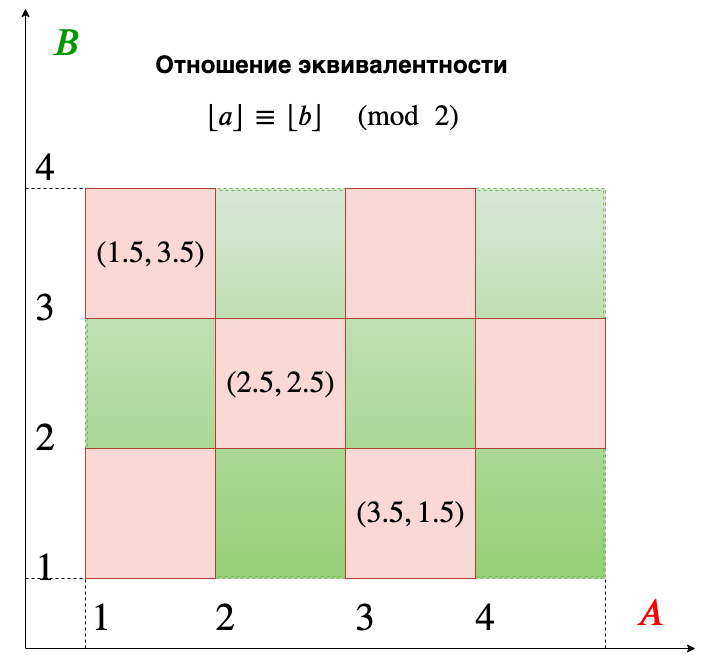
\includegraphics[scale=0.25]{equiv.png}
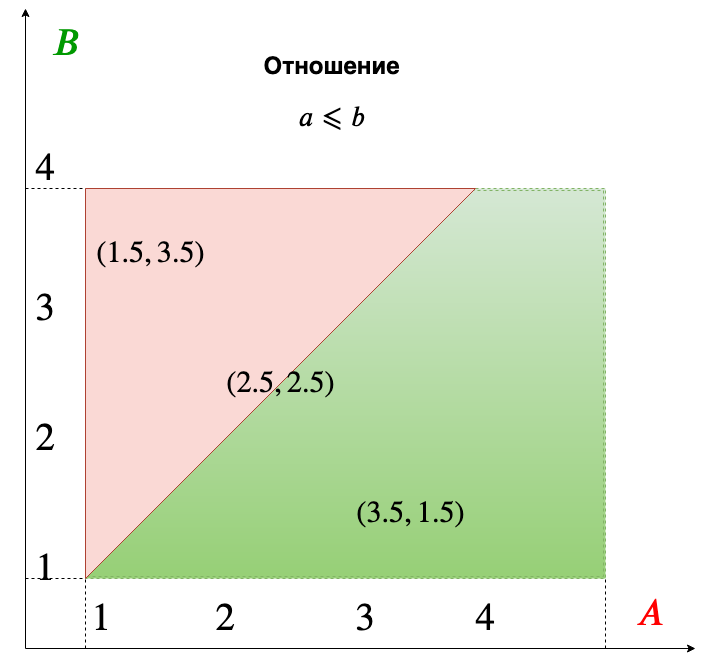
\includegraphics[scale=0.25]{lessthan.png}
\end{center}


\section{Числа Гаусса}

\subsection{Конспект}
\begin{enumerate}\setlength{\itemsep}{1pt}
\item 
\item 
\item 
\item 
\item 
\item 
\item 
\item 
\item 
\item 
\end{enumerate}
\subsection{Задачи}



\newchapter{Числовые поля}

\section{Рациональные дроби}

\subsection{Конспект}
\begin{enumerate}\setlength{\itemsep}{1pt}
\item 
\item 
\item 
\item 
\item 
\item 
\item 
\item 
\item 
\item 
\end{enumerate}
\subsection{Задачи}



\section{Цепные дроби}

\subsection{Конспект}
\begin{enumerate}\setlength{\itemsep}{1pt}
\item 
\item 
\item 
\item 
\item 
\item 
\item 
\item 
\item 
\item 
\end{enumerate}
\subsection{Задачи}



\section{Расширение поля рациональных чисел}

\subsection{Конспект}
\begin{enumerate}\setlength{\itemsep}{1pt}
\item 
\item 
\item 
\item 
\item 
\item 
\item 
\item 
\item 
\item 
\end{enumerate}
\subsection{Задачи}




\section{Комплексные числа}

\subsection{Конспект}
\begin{enumerate}\setlength{\itemsep}{1pt}
\item 
\item 
\item 
\item 
\item 
\item 
\item 
\item 
\item 
\item 
\end{enumerate}
\subsection{Задачи}



\section{Реализация движений с помощью комплексных чисел}

\subsection{Конспект}
\begin{enumerate}\setlength{\itemsep}{1pt}
\item 
\item 
\item 
\item 
\item 
\item 
\item 
\item 
\item 
\item 
\end{enumerate}
\subsection{Задачи}



\section{Гомотетии прямой и плоскости}

\subsection{Конспект}
\begin{enumerate}\setlength{\itemsep}{1pt}
\item 
\item 
\item 
\item 
\item 
\item 
\item 
\item 
\item 
\item 
\end{enumerate}
\subsection{Задачи}




